\scanpage{24}
% archive foliation: 23
Ceci fait, regardons, pour un $G$ quasi-cohérent
variable sur $S_0$, les $\unsure{q_*}\underline{\operatorname{Hom}}(,\underline{O}_{\unsure{\Gamma_0|P_0}}\otimes_{S_0}G)$,
$\unsure{q'_*}\underline{\operatorname{Hom}}(,\underline{O}_{\unsure{\Gamma'_0|P'_0}}\otimes_{S_0}G)$
relatifs aux deux lignes, on trouve un
\inserted{(si les Hom sont \uline{représentatifs})}
diagramme commutatif de suites exactes
\[
(D)\quad
\diagram{\begin{tikzcd}
&L\arrow[r,"i"]&M\arrow[r,"d"]&N\arrow[r]&0\\
0\arrow[r]&L'\arrow[u,"\alpha"]\arrow[r,"i'"]&M'\arrow[u,"\beta"]\arrow[r,"d'"]&N'\arrow[u,"\gamma"]\arrow[r]&0
\end{tikzcd}},
\]
de plus on a un hom. can. $\sigma$
\figure{\begin{tikzpicture}
\node[inner sep=0] at (0,0) {\diagram{\begin{tikzcd}[ampersand replacement=\&,column sep=2.2em,row sep=2em]
\&L\arrow[dl,"\sigma"']\\J\arrow[d,dashed,"\unsure{\lambda}"']\&L'\arrow[u,"\alpha"]\\G\&
\end{tikzcd}}};
\draw (-1.15,0.1)--(0.25,1.55)--(1.05,1.28);
\draw (1.04,1.05)--(-0.72,-0.28)--(-1.05,0.02);
\end{tikzpicture}}
\diagram{\begin{tikzcd}L'&M'\arrow[l,"\pi'"']\end{tikzcd}}
correspondant à l'identité
$\underline{O}_{\Gamma_0}\otimes_{S_0}J\longrightarrow\underline{O}_{\Gamma_0}\otimes_{S_0}\underset{=G}{J}$,
et un \uline{splittage} \inserted{$M'\xrightarrow{\unsure{\pi|\pi'}}L'$} de la deuxième ligne.
Ceci dit, pour un $\lambda:J\longrightarrow G$ donné,
les solutions du pb relatif à $G$ sont
les hom $M\xrightarrow{\mu}G$ qui \uline{relèvent}
le composé $L\xrightarrow{\lambda\sigma}G$, \inserted{i.e. $\boxed{\mu i=\lambda\sigma}$}, et tels que
$\mu\beta=(\lambda\sigma\alpha)\pi'$. \deleted{\unsure{Il}} Pour qu'il en existe un
il f. et s. que
\[
1^\circ)\quad (\lambda\sigma)(\operatorname{Ker}i)=0\quad\text{i.e.}\quad
\lambda(R_1)=0,\quad\text{où}\quad R_1=\sigma(\operatorname{Ker}i)\subset J
\]
\deleted{[i.e. $\lambda$ se factorise en $\bar\lambda:\bar J=J/\unsure{K}\longrightarrow G$]}
\margin{Alors on peut remplacer $L$ par $L/\operatorname{Ker}i$.}
\margin{\figure{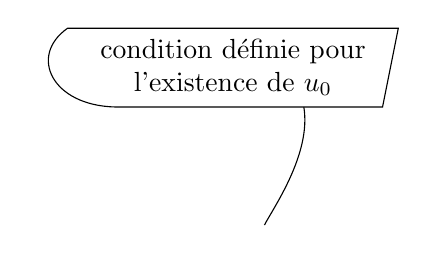
\begin{tikzpicture}[baseline=(m.base)]
\node[text width=4cm,align=center,inner sep=2pt] (m) at (0,0) {\unsure{condition définie pour l'existence de} $u_0$};
\draw (-2.1,0.5)..controls(-2.6,0.15)and(-2.3,-0.48)..(-1.5,-0.5)--(1.9,-0.5)--(2.1,0.5)--cycle;
\draw (0.9,-0.5)..controls(1,-1.1)and(0.5,-1.8)..(0.4,-2);
\end{tikzpicture}}}
$2^\circ)$ [Tenant compte que \uline{$\gamma$ est surjectif}]
$\lambda\sigma\alpha\pi'$ \unsure{s'annule} sur \deleted{\unsure{$R_2=$}} $\operatorname{Ker}\beta$,
i.e. $\lambda(R_2)=0$; où $R_2=\sigma\alpha\pi'(\operatorname{Ker}\beta)$.
